\documentclass[a4paper,10pt,twoside]{report}

\usepackage[margin=1in]{geometry}
\usepackage{amsmath}
\usepackage{titling}
\usepackage{fontspec}
\usepackage{listings}
\usepackage{hyperref}
\usepackage{graphicx}

\usepackage[dvipsnames]{xcolor}

\lstdefinelanguage{Java}{
	keywords=[1]{
		fields, schemaData, dataframe, latMin, latMax, longMin, longMax, rightOuter, leftOuter, lat1, lon1, lat2, lon2, deltaLat, deltaLon, c, d, a, radius, distance, time, tokenizer, remover, assembler, linreg, rfr, trainsetsplit, traintestsplit, indexer, minmax, pipelinerfr, paramgridrfr, pipelinelinreg, trainedlinreg, model, cvmrfr, evaluator, calc, log, metrictype, metrictypes, svc, pca, paramgridsvm, cvsvm, predictionssvm, metrics, predictionsLogReg, predictions, train, test, trainsetsplit, traintestsplit, datasets, createsubsample, pipelinesvm, glr, paramgridglr, gbt, paramgridgbt, pipelineglr, pipelinegbt, predictionsrfr, cvrfr, trainvalidationsplitglr, trainvalidationsplitgbt, range, nietfraudulent, lengte, arrfeatures, kolom, creditcardsubsample, cvmSVM, trainingset, testset, matrix, r1, vectorizer, lr, paramgridlogreg, pipelinelogreg, htf, rfc, paramgridrfc, cvrfc, pipelinerfc, pipelinemodellogreg, predictedlogreg, predictionsrfc},
	keywordstyle=[1]\color{Bittersweet},
	keywords=[2]{linearsvc, pipeline, parammap, minmaxscaler, vectorassembler, crossvalidatormodel, linearregression, pipelinemodel, stringindexer, randomforestregressor, crossvalidator, regressionevaluator, regextokenizer, stopwordsremover, countvectorizer, hashingtf, logisticregression, paramgridbuilder, randomforestclassifier}, % ML-typen
	keywordstyle=[2]\color{purple},	
	keywords=[3]{private, static, final, throws, public, exception, call, udf4, udf2, new, return, system, printf}, 
	keywordstyle=[3]\color{violet},
	keywords=[4]{double, doubletype, timestamptype, stringtype, integertype, boolean , int, long, string, dataset},
	keywordstyle=[4]\color{RoyalBlue},
	keywords=[5]{label, prediction, verhouding, metric, spark},
	keywordstyle=[5]\color{Aquamarine}\bfseries,
	keywords=[6]{getTraining, getTest, clean, haversine, speed, printcorrelation, getarearoccurve, printconfusionmatrixmetrics, printregressionevaluation, getrangedataframe, getdata, createsubmission, adddistance, addspeed},
	keywordstyle=[6]\color{OliveGreen}\bfseries,
	keywords=[7]{where, select, first, orderby, groupby, count, show, drop, mean, sum, fit, transform, randomsplit, getdouble, withcolumn, union, sample, columns, weightedprecision, weightedrecall, accuracy},
	keywordstyle=[7]\color{PineGreen},
	keywords=[8]{pickuplatitude, pickuplongitude, dropofflatitude, dropofflongitude}, %input
	keywordstyle=[8]\color{Periwinkle},
	identifierstyle=\color{black},
	sensitive=false,
	comment=[l]{//},
	morecomment=[s]{/*}{*/},
	commentstyle=\color{red}\ttfamily,
	stringstyle=\color{Sepia}\ttfamily,
	morestring=[b]',
	morestring=[b]"
}

\lstset{ %
	backgroundcolor=\color{white},   
	basicstyle=\footnotesize,        
	breakatwhitespace=false,         
	breaklines=true,                 
	captionpos=b,                    
	commentstyle=\color{commentsColor}\textit,
	deletekeywords={...},            % if you want to delete keywords from the given language
	escapeinside={\%*}{*)},          % if you want to add LaTeX within your code
	extendedchars=true,              % lets you use non-ASCII characters; for 8-bits encodings only, does not work with UTF-8
	frame=tb,	                   	   % adds a frame around the code
	keepspaces=true,                 % keeps spaces in text, useful for keeping indentation of code (possibly needs columns=flexible)
	keywordstyle=\color{keywordsColor},       % keyword style
	language=Python,                 % the language of the code (can be overrided per snippet)
	otherkeywords={*,...},           % if you want to add more keywords to the set
	numbers=left,                    % where to put the line-numbers; possible values are (none, left, right)
	numbersep=5pt,                   % how far the line-numbers are from the code
	numberstyle=\tiny\color{commentsColor}, % the style that is used for the line-numbers
	rulecolor=\color{black},         % if not set, the frame-color may be changed on line-breaks within not-black text (e.g. comments (green here))
	showspaces=false,                % show spaces everywhere adding particular underscores; it overrides 'showstringspaces'
	showstringspaces=false,          % underline spaces within strings only
	showtabs=false,                  % show tabs within strings adding particular underscores
	stepnumber=1,                    % the step between two line-numbers. If it's 1, each line will be numbered
	stringstyle=\color{stringColor}, % string literal style
	tabsize=2,	                   % sets default tabsize to 2 spaces
	title=\lstname,                  % show the filename of files included with \lstinputlisting; also try caption instead of title
	columns=fixed                    % Using fixed column width (for e.g. nice alignment)
}

\newfontfamily\headingfont[]{Montserrat-Black}

\usepackage[dutch]{babel}

\usepackage{fontspec}
\setmainfont{Montserrat}

\title{Samenvatting Distributed Databanken}

\author{Dylan {Cluyse}}
\begin{document}
	
\maketitle

\tableofcontents
	
\chapter{Gedistribueerde databanksystemen}

\section{Inleiding}

\subsection{Breed beeld}

Een gedistribueerd bestandssysteem is een manier om gegevens op te slaan en te beheren die is verspreid over meerdere computers in een cluster. In tegenstelling tot een traditioneel bestandssysteem, waarbij de gegevens op één centrale server worden opgeslagen, worden de gegevens in een gedistribueerd bestandssysteem opgeslagen op verschillende computers in het cluster. Dit maakt het mogelijk om grote hoeveelheden gegevens op te slaan en te verwerken zonder te worden beperkt door de beperkte hoeveelheid opslagruimte op één server. Het kan ook helpen om de prestaties te verbeteren door het gebruik van parallellisatie, waardoor meerdere computers tegelijkertijd kunnen werken aan het verwerken van de gegevens.

\begin{itemize}
	\item Verschillende componenten op een netwerk die met elkaar communiceren.
	\item Een systeem met het doel om data beschikbaar te maken. Data dat later kan worden gelezen of geschreven.
	\item De mate van beschikbaarheid doet er niet toe.
\end{itemize}

\subsection{De nood aan schaalbaarheid}

In een gedistribueerd bestandssysteem is er een verschil tussen horizontale en verticale schaalbaarheid. Horizontale schaalbaarheid betekent dat het systeem kan worden uitgebreid door het toevoegen van meer computers aan het cluster, wat kan helpen om meer gegevens te verwerken en om de prestaties te verbeteren. Verticale schaalbaarheid betekent dat het systeem kan worden uitgebreid door het toevoegen van meer hardware aan een enkele computer, zoals extra geheugen of een snellere processor. Dit kan ook helpen om de prestaties te verbeteren, maar het is beperkter dan horizontale schaalbaarheid omdat het alleen mogelijk is binnen de beperkingen van een enkele computer.

Moore's Law bevestigt deze theorie. Deze wet zegt dat het aantal transistoren per achttien maanden verdubbelt. Met andere woorden is er een snelle nood aan nieuwe hardwarematerialen. Daarnaast is er ook nood aan nieuwe hardwarematerialen, zo is er nood aan fouttolerantie in een databankomgeving. 

Het verkeer bij een databankserver gebeurt online, wat betekent dat de latency een rol speelt voor de gebruiker. De client moet een systeem kiezen die zo dicht mogelijk bij de client ligt. Online gameservers zijn een goede casus waarbij de systemen opgedeeld zijn per regio.

\subsection{Kenmerken}

Een gedistribueerd systeem kan herkend worden op basis van vier kenmerken:

\begin{itemize}
	\item Geen gedeeld geheugen. Iedere verwerkingseenheid heeft een eigen geheugen.
	\item Onderling worden er berichten naar elkaar verstuurd.
	\item Componenenten zijn niet bewust van wat de andere componenten nu aan het doen zijn. Daarom sturen ze onderling berichten naar elkaar.
	\item Fouttolerant
\end{itemize}

\section{Soorten systemen}

We spreken van twee verschillende soorten systemen: parallele en gedistribueerde systemen.

\begin{itemize}
	\item Bij een parallel systeem worden meerdere processen tegelijkertijd uitgevoerd. Deze verwerking gebeurt op verschillende verwerkingseenheden met een gedeeld geheugen. Het is makkelijker te ontwikkelen, maar met de kost van géén redundantie.
	\item Een gedistribueerd systeem bevat verschillende verwerkingseenheden met elk een eigen geheugen. De andere componenten zijn onbewust van wat de andere onderdelen aan het doen zijn. Er wordt onderling berichten met elkaar verstuurd. Dit noemt ook een shared-nothing architecture: Er wordt niets onderling gedeeld. De enige manier van communicatie is door middel van boodschappen.
\end{itemize}

\subsection{CAP-theorem}

Deze theorie wijst aan dat je, in een gedistribueerd databanksysteem, de afweging moet maken tussen drie factoren:

\begin{itemize}
	\item Consistentie wijst aaan dat alle nodes dezelfde gegevens hebben.
	\item Beschikbaarheid wijst aan dat het systeem beschikbaar blijft voor alle gebruikers, zelfs al is er een crash of een paar nodes die niet beschikbaar zijn.
	\item Partitioneringstolerantie wijst aan dat het systeem blijft functioneren als er problemen zijn met de communicatie tussen de nodes.
\end{itemize}

Het is onmogelijk om alle drie deze eigenschappen tegelijkertijd te garanderen. Je moet een afweging maken of compromis sluiten.

Deze stelling komt terug uit databanken, maar hier is het anders. De consistentie van een relationele databank overstijgt de consistentie van een gedistribueerde databank.

\subsection{Struikelblokken}

Als we werken met een gedistribueerd systeem, dan zijn er vier horden waarmee we rekening moeten houden:
* Split-brain scenario: de ene helft denkt het ene en de andere helft denkt het andere. Bijvoorbeeld: Het ene systeem denkt dat een bestand verwijderd is, terwijl het andere systeem denkt dat het nog bestaat.
* Consistency en structuur raken snel verloren.
* Testen wordt moeilijker.
* De oorzaak van traagheid achterhalen wordt complexer: zowel hardware als software kunnen een rol spelen.

\subsection{Fabels over gedistribueerde systemen}


\begin{itemize}
	\item "Er is geen latency". Latency is wel aanwezig. Enkel is de deze sterk minder naargelang de locatie van het systeem. het duurt een tijd vooraleer een bericht op een systeem aankomt.
	\item "De bandbreedte is oneindig". De bandbreedte op zowel de client als het distribueerd systeem is beperkt.
	\item "Het netwerk is veilig". Toegang tot het netwerk blijft iets waar je rekening mee moet houden.
	\item "De netwerktopologie blijft hetzelfde". Computers en hardware kan worden toegevoegd. Zo verandert alles binnen een netwerk op een dynamische manier.
	\item "De transportkost van data is nul". Data transporteren van begin- naar eindpunt vergt een inspanning qua energie en rekenkracht.
	\item "Het netwerk is homogeen". Alle onderdelen binnen een netwerk kunnen variëren van eigenschappen. Sommige delen van het netwerk kunnen snel zijn, sommige delen zijn traag.
\end{itemize}

\section{Problemen met gedistribueerde netwerken}

Bij een gedistribueerd systeem zijn er vier algemene problemen:

\begin{itemize}
	\item Partial failures
	\item Niet-betrouwbare netwerken
	\item Niet-betrouwbare tijdsindicaties
	\item Onderlinge onzekerheid
\end{itemize}

\subsection{Partial Failure}

Er moet rekening worden gehouden met twee zaken: 

\begin{itemize}
	\item Allereerst is er de kans dat een systeem kan wegvallen. Sommige onderdelen van een netwerk kunnen werken, terwijl andere onderdelen down zijn of niet meer in gebruik. Hoe meer computers, hoe groter de kans dat één systeem (heel even) wegvalt.
	\item Als tweede punt kunnen andere systemen niet zien wanneer een systeem wegvalt. Het probleem wordt pas opgemerkt wanneer er geen antwoord is. De oorzaak kennen we niet. Dit kan liggen aan: overbelasting, defunct, te traag vergeleken met andere systemen, etc.
\end{itemize}

\subsection{Niet-betrouwbare netwerken}

Bij een asynchrone verbinding moeten we rekening houden met tijdsaannames. Boodschappen worden verstuurd zonder tijdsaannames. Het maakt de systemen niet uit hoe lang ze moeten uitvoeren of wanneer het bericht zal arriveren. De oorzaak van een netwerkfout is hier niet voor de hand liggend. Het is moeilijk om de oorzaak te achterhalen, want er zijn drie mogelijke problemen: een probleem tussen zender en ontvanger, de ontvanger kan niets ontvangen of de ontvanger kan niets versturen.

Het testen van een verbinding gebeurt met \textit{pinging}. Om te vermijden dat een systeem iedere twee seconden een test uitvoert, werken we met \textit{exponential back-off}. De tijd waarop een systeem wacht op een antwoord moet exponentieel vergroten. Begin met twee seconden wachten, daarna vijf seconden, daarna tien seconden, ... tot maximaal vijf minuten. Te snel berichten sturen moet vermeden worden, want zo wordt het netwerk belast en dan verergert de situatie. Eenmaal de capaciteit van de wachtrij wordt behaald, dan zal de vertraging (in seconden) exponentieel verhogen. IRL-voorbeeld: files.

\subsection{Niet-betrouwbare tijdsindicaties}

Er wordt het onderscheid tussen real-time en monotonische tijd gemaakt. 

\begin{itemize}
	\item Real-time tijd zijn klokken die gesynchroniseerd worden met het gebruik van een gecentraliseerde server.
	\item Monotonische klokken zijn klokken die op een vast moment starten en enkel vooruit gaan. Er is geen synchronisatie. Leap-seconden: een minuut is niet altijd 60 seconden. Soms kan dit 59 of 61 seconden zijn.
\end{itemize}

Causality is achterhalen wanneer een event werd uitgevoerd. Concensus is wanneer alle knopen (of nodes) met elkaar overeenkomen bij een beslissing.

\subsection{Onderlinge onzekerheid}

Nodes in een gedistribueerd systeem kan enkel veronderstellingen maken. De informatie dat een node bijhoudt verandert regelmatig. Voorbeelden hiervan zijn: klokken die desynchroniseren of nodes die niets terugsturen terwijl ze een update uitvoeren.

Split-brain is een concept rond inconsistente data-opslag. De ene helft van het systeem denkt dat iets juist is, terwijl de andere helft van het systeem denkt dat iets anders juist is. Bijvoorbeeld deel A denkt dat systeem 1 de baas is, terwijl deel B denkt dat systeem 2 de baas is.

Het tweegeneralenprobleem bouwt verder op het split-brain concept. Dit weergeeft een scenario waarin beide partijen enkel winnen als ze samenwerken. Elk ander scenario leidt tot verlies. Beide partijen weten niet of de andere partij iets wilt ondernemen. Ze moeten het eerst vragen. De boodschap kan mogelijks niet tot de generaal komen.

Dit probleem kunnen we toepassen binnen een online webshop. Er zijn drie gevallen:

| Online shop | Payments service | Resultaat |
| -- | -- | -- |
| verzendt het pakket niet | vraagt geen geld | / |
| verstuurt het pakket | vraagt geen geld | de shop is hier nadelig |
| verzendt het pakket niet | vraagt geld | de klant is hier nadelig |
| verstuurt het pakket | vraagt geld | :D |

\section{Replication en partitioning}

\subsection{Partitionering}

Bij partitionering zal je een groot bestand onderverdelen over meerdere knopen. Op deze manier hoef je niet alles op één plek op te slaan. Het nadeel hiervan is dat je geen toegang hebt tot het volledige bestand als één van de nodes niet bereikbaar is. Elk stuk data behoort tot precies één partitie. Bij Mongo en ElasticSearch noemt één partitie een \textit{shard}.

\subsection{Replication}

Replicatie is het maken en onderhouden van verschillende kopieën op meerdere knooppunten. Hiermee wordt redundantie aangeboden. Als de data op node A niet beschikbaar is, dan worden gebruikers doorverwezen naar node B. Dit concept komt vaak voor bij geografisch gespreide netwerken. Bijvoorbeeld een knooppunt in Oceanië, Azië, Europa, etc. Er zijn hier drie verschillende leader-volger technieken: 

\begin{enumerate}
	\item  Bij single-leader doen alle clients wat de leider zegt. Alle writes komen vanuit één leider binnen één partitie. De boodschap van de clients kan gedateerd zijn. Als gevolg kunnen acties uitgevoerd worden die niet meer van toepassing zijn. 
	\item Bij leaderless replication versturen de clients elke write naar verschillende nodes. De clients lezen parallel.  Zij zorgen ervoor dat de data OK blijft. Elk verstuurt boodschappen door naar de nabije clients. Achterhaalde data kan worden tegengegaan door te werken met timestamps.
	\item  Multi-leader replication bouwt verder op single-leader replication. Meerdere nodes worden in verschillende datacenters geplaatst.
\end{enumerate}

\subsection{Replication-lag}

Leaders zijn niet statisch. Deze kunnen veranderen door clients te promoveren tot leader. Als een leader verandert, dan is er de kans op replication-lag. Dit is wanneer een volger wordt gepromoveerd tot leader.

Replication kan synchroon of asynchroon verlopen. Synchroon is wanneer je wacht op de antwoorden van de volgers. Je bent hiermee zeker dat de data niet zal verloren gaan, maar ten gevolge zal het systeem trager zijn. Asynchroon is wanneer er niet wordt gewacht op de volgers. Alle overplaatsingen zullen vlot verlopen als er geen wissels gebeuren bij de leaders. Hoe groter de replication lag, hoe groter de kans op dataverlies.
 
\begin{figure}
 	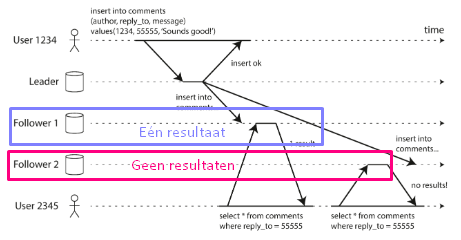
\includegraphics[width=\linewidth]{../images/Screenshot_213.png}
 	\caption{Het verschil tussen synchrone en asynchrone replication. Bij synchroon wacht je niet op bevestiging. Synchrone replicatie gaat direct door naar de target storage. Asynchrone replication wacht op bevestiging van de volgers op de source.}
\end{figure}

\subsection{Replicatiefouten}

Fouten bij synchrone replicatie zijn minder voorkomend, maar de techniek kan gedwarsboomd worden. Zo heb je nog steeds een probleem wanneer een write-operation niet kan worden afgewerkt als één van de volgers niet online is. Je wacht tot de bevestiging van de volgers.

\begin{figure}
	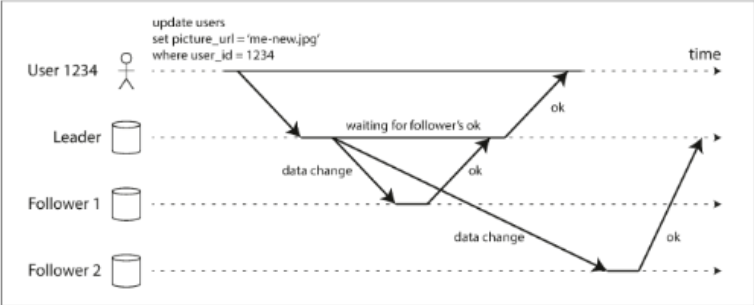
\includegraphics[width=\linewidth]{../images/Screenshot_160.png}
	\caption{Voorbeeld van een fout bij synchrone replicatie.}
\end{figure}

De twee vaak voorkomende fouten bij asynchrone replicatie zijn monotonic read en read-after-write. 

\begin{itemize}
	\item Read-after-write (RAW) duidt, zoals de naam het aangeeft, op een fout bij het lezen. De client heeft in dit geval een comment geplaatst en vervolgens wordt er een bevestiging gegeven aan de client. Daarna wilt dezelfde gebruiker dezelfde post inlezen, maar die is nog niet opgeslaan door een andere volger. Je wilt dezelfde output krijgen als je hetzelfde in de databank schrijft. Bij RAW is het belangrijk om met een timestamp te werken. Zorg dat je bij een schrijfoperatie alles tot aan een punt moet laten voldoen aan de timestamp. Zo ja, haal de gegevens op en geef ze aan de client. Zo niet, wacht of kijk naar een andere volger.
	\item Een gelijkaardig, maar nog steeds verschillend probleem, is monotonic read. De gebruiker leest een post of comment, maar na een refresh is deze comment opeens niet beschikbaar of niet-bestaand. De volger loopt hier achter op de andere volgers. De klok bij de ene volger loopt voor op de andere. Het verschil hier is dat de gebruiker de tekst niet heeft geschreven, wat wel het geval is bij RAW. Dit lossen we op door de gebruiker altijd van dezelfde replica te laten lezen. Hieronder leest de gebruiker eerst van de volger mét het resultaat. Daarna probeert de gebruiker dit opnieuw, maar bij een volger die achterloopt.
\end{itemize}


\begin{figure}
	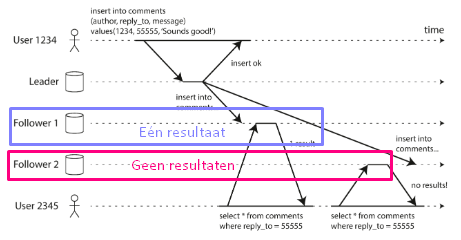
\includegraphics[width=\linewidth]{../images/Screenshot_213.png}
	\caption{Monotonic read}
\end{figure}

\begin{figure}
	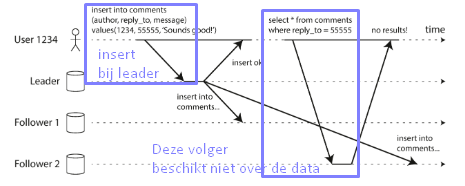
\includegraphics[width=\linewidth]{../images/Screenshot_214.png}
	\caption{Read-after-write probleem.}
\end{figure}

\subsection{Replicatie en partitionering combineren}



\begin{figure}
	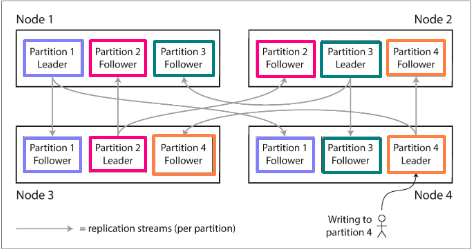
\includegraphics[width=\linewidth]{../images/Screenshot_215.png}
	\caption{Vier partities: elke leader heeft twee volgers. In de volgende foto zijn er vier nodes. Elke node heeft drie onderdelen. Over de vier nodes zijn er vier verschillende partities verdeeld. De replica's of volgers kan je achterhalen aan de hand van de stream. De leider van partitie 1 in node 1. De replica's zijn in Node 3 en in Node 4. De leider van partitie 2 is in node 3. De replica's zijn in Node 1 en in Node 2.}
\end{figure}

We kunnen niet zomaar data in stukken snijden. We moetne hotspots vermijden. Een hotspot is een plaats waar de verdeling geen goede verhouding heeft voor iedere node. Hiervoor hebben we twee oplossingen: key-value partitionering en hash partitionering.

\begin{itemize}
	\item Key-value partitionering is wanneer je een zo eerlijk en even mogelijke verdeling maakt over alle nodes. Alle sleutels binnen een node behoren tot een range. Je sorteert alle sleutels. Bijvoorbeeld alles van A t.e.m. E. Afhankelijk van de context wordt vaak voorkomende data binnen dezelfde partitie opgeslaan. Dit zorgt voor meer verkeer op partitie A-D vergeleken met X-Z. De ene partitie zal een hotspot worden, maar de andere zal geen verkeer krijgen.
	\item Hash partioning lost dit probleem merendeels op, maar het is niet de meest efficiënte implementatie. Hier verlies je sortering. De compromise hier is dat je wél een even verdeling zal krijgen. De hash houdt rekening met beschikbare plaats. De kans dat een partitie niet gebruikt zal worden is kleiner. 
\end{itemize}


\section{Request routing}

De plaats van data achterhalen kan op drie manieren:

1. Iedere node bevat metadata. De client kan een willekeurige knoop contacteren. De knoop weet waar het te zoeken woord is. Hieronder geeft knoop 0 mee dat het te zoeken woord op knoop 2 is.

2. Er is een laag tussen de client en de knopen. De routing-tier bevat metadata.

3. De client heeft directe toegang tot de metadata. Dit wordt het minste gebruikt.

\begin{figure}
	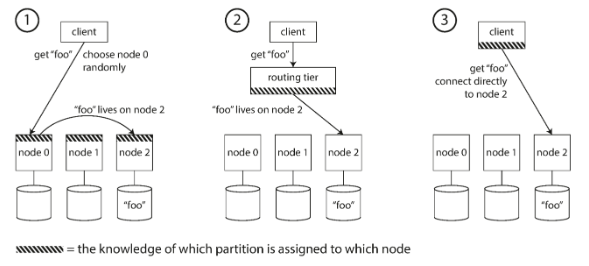
\includegraphics[width=\linewidth]{../images/Screenshot_216.png}
	\caption{De drie mogelijkheden om de plaats van data te achterhalen.}
\end{figure}

De locatie van metadata onderhouden gebeurt met de coordination service. Dit zorgt voor het onderhoud en de mapping van de metadata. Het is de routing tier (RT) tussen de client en de knopen. De RT is direct verbonden met zowel de knopen, alsook met de Zookeeper. Als er iets verandert in de data van een node, dan meoten de nodes dit laten weten aan de Zookeeper.

\begin{figure}
	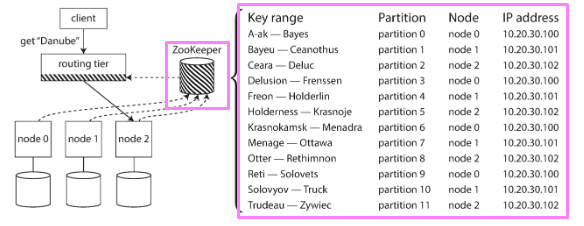
\includegraphics[width=\linewidth]{../images/Screenshot_217.png}
	\caption{Zookeeper.}
\end{figure}

\chapter{Hadoop Filesystem}

\section{Inleiding}

Het maakt gebruik van parallellisatie om de gegevens te verdelen over meerdere computers in een cluster, waardoor het verwerkingsproces sneller wordt. Dit kan worden gebruikt voor het analyseren van gegevens, zoals het ontdekken van trends en patroonherkenning. Hadoop is één van de eerste frameworks voor Big Data Processing. Het is een relatief oud project met *clunky* technieken. 

Het is ontworpen met de gedachten om clusters te kunnen draaien op normale hardware. Als je cluster bestaat uit honderden computers, dan is de kans groot dat er één zal breken. Het basisidee van Hadoop is om dit soort fouten af te handelen en zodat het systeem blijft werken zoals voordien.

\subsection{Hadoop stack}

Een pure hadoop-stack bestaat uit vier onderdelen:
* Hadoop common: de gedeelde bibliotheken die door de andere modules worden gebruikt. Je ziet dit gedeelte niet. Het is de meeste onderste laag.
* HDFS is een filesystem. Dit zorgt voor de distributed file storage. Je merkt de delay amper.
* MapReduce is het processing-gedeelte. MapReduce laat je toe om parallel grote datasets te verwerken.
* YARN voorkomt dat één element in je cluster alle resources opeet. Dit element zorgt voor request-afhandeling van resourcevragen.

\section{Hadoop filesystem}

\subsection{Designprincipes}

Een filesystem laat toe om data op te slaan en weer op te halen. Er zijn drie soorten data: files, mappen en metadata. Metadata is de info over de mappen of bestanden, zoals file length en permissies. Een filesystem zorgt ervoor dat de data toegankelijk is. De consistentie in filesystems wordt bewaard door middel van een logsysteem. 

De data wordt opgeslaan in een cluster van gewone machines. De focus van HDFS ligt op riante hoeveelheden data op te slaan. Er wordt gewerkt met veel groepen van machines. Als er één machine zou kapot gaan, dan neemt een andere machine over. Er is weinig vertraging.

Write-once-read-many-times (WORM) betekent dat gegevens één keer worden geschreven en vervolgens vele keren worden gelezen, maar niet wordt gewijzigd of verwijderd. HDFS ondersteunt deze techniek om zo een hoge fouttolerantie te kunnen bieden en doorvoer te kunnen bieden. 

Er zijn verschillende redenen waarom er geen bestanden worden gewijzigd of verwijderd.

\begin{itemize}
	\item HDFS is bedoeld om grote hoeveelheden data op te slaan. Verwijderen en wijzigen vergt kostbare energie. Daarnaast is HDFS fouttolerant, want het systeem moet blijven werken zelfs al vallen er nodes uit. Als een bestand wordt verwijderd, dan beïnvloedt dit de integriteit van de data.
	\item HDFS is bedoeld om een historiek uit te bouwen. De data wordt ingezet in data-analyse, waar nauwkeurigheid een rol speelt, dus er mogen geen wijzigingen aan de data worden aangebracht.
\end{itemize}

Het principe is 'write-once, read-many-times'. Een bestand wordt eenmalig gemaakt. De doorvoer van het systeem is hier belangrijker. De hoeveelheid verwerkte data per tijdseenheid. HDFS op een klassiek filesysteem. Eens de machine bezig is kan je een grote doorvoer hebben. 

Er is sprake van \textbf{append-only fashion}. De gegevens kunnen enkel achteraan worden toegevoegd en niet tussenin of helemaal vooraan. Deze werkwijze helpt om de prestaties en betrouwbaarheid van HDFS te verbeteren, omdat het aantal wijzigingen aan gegevens beperkt. 

\subsection{Anti-patterns}

Er zijn enkele situaties waarbij HDFS \textit{overkill} of ongeschikt is als oplossing:

\begin{itemize}
	\item Wanneer snelheid een grote rol speelt. De latency is hier niet minimaal.
	\item Wanneer het merendeel van de data uit kleine bestanden bestaat. De nadruk bij HDFS ligt op grote bestanden. De NameNode houdt de directorystructuur bij, waardoor veel kleine bestanden zal leiden tot veel verschillende takken.
	\item Wanneer je meerdere schrijvers op eenzelfde moment wilt hebben. Als één client schrijft en de andere wilt lezen, dan kan er een conflict ontstaan bij de integriteit en het delen van een bestand.
	\item Wanneer je gegevens
\end{itemize}

* Append-only fashion: Als je inhoud vooraan of in het midden wilt toevoegen.


\subsection{Hadoop-onderdelen}

HDFS heeft twee componenten:

\begin{itemize}
	\item De NameNode.
	\item De DataNode.
\end{itemize}

Kort samengevat is de namenode de node dat het bestandssysteem beheert en bijhoudt waar alle bestanden zijn opgeslagen. De datanode slaat de bestanden op en zorgt ervoor dat gegevens beschikbaar zijn voor lezen en schrijven.

\subsection{NameNode}

Een NameNode (NN) weet uit welke blokken de data bestaat en houdt bij op welke datanodes de blokken staan. Locaties worden niet persistent bijgehouden. Onderling weten ze dit door middel van \textit{heartbeats}.  Als je een file wilt hernoemen, dan lukt dat ook. Bij een cluster heb je altijd één NN.

Dit is één computer die de filesystem-namespace zal managen. Die houdt bij wat de metadata is, de structuur van de directory. Metadata wordt in het RAM bijgehouden. Het is snel, maar vluchtig. De informatie moet worden bijgehouden.

1.  
1.1. De NameSpace Image is de directory structuur, dus alles met de inhoud van de directory. Terwijl het systeem loopt wordt het opgebouwd.
1.2. De edit logs: Dit is een append-log. Telkens als er iets verandert komt er informatie bij. Als de NN opnieuw zou opstarten, dan wordt de image en edit log gelezen. Daarna worden de veranderingen van de edit log toegepast op de namespace image om zo een nieuwe namespace image te maken. Daarna wordt een nieuwe edit log gestart.

\subsection{DataNode}

Waar wordt de datablokken opgeslaan? 
Op een DataNode. Als je iets leest is het altijd direct op de DataNode. De DN's luisteren direct naar de NN. Elk blok heeft een replicatiefactor. De replicatiefactor wijst op hoeveel systemen het bestand beschikbaar moet staan. Een HDFS heeft veel DataNodes.

\section{Single-point-of-failure}

Als één NN uitvalt, of als de NS Image uitvalt, dan heb je een probleem. Je systeem werkt niet meer. Je zal alle data nog hebben op de DN. Alle blokken hebben random verwijzingen. Je weet niet meer waarvan de data komt of waarnaar de data gaat.

De meest voor de hand liggende manier is om regelmatig een backup te nemen. In praktische systemen
De tweede optie is een secondary NN. Zolang je een systeem niet herstart wordt je edit log langer en groter. Dit is niet ideaal, want als het neemt zowel plaats in alsook zal het opstarten van een NS image langer duren. In latere versie van Hadoop hebben ze een secondary NN toegevoegd. Een secondary NN is een proces dat op een andere computer loopt en dat de veranderingen van de edit log verwerkt in de huidige namespace.

\section{MapReduce}

Hadoop MapReduce is een programma dat wordt gebruikt voor het verwerken van grote hoeveelheden gegevens in een distributiefile-systeem. Het maakt gebruik van parallellisatie om de gegevens te verdelen over meerdere computers in een cluster, waardoor het verwerkingsproces sneller wordt. Dit kan worden gebruikt voor het analyseren van gegevens, zoals het ontdekken van trends en patroonherkenning. Een MapReduce bestaat uit drie fasen:

\begin{enumerate}
	\item Mapping
	\item Shuffle
	\item Reduce
\end{enumerate}

\subsection{Mapping}

De Mapper in Hadoop MapReduce is een programma dat wordt gebruikt om gegevens te verdelen over meerdere computers in een cluster, zodat ze parallel kunnen worden verwerkt. De Mapper leest de gegevens in en verdeelt ze in kleinere stukjes, die vervolgens naar de verschillende computers in het cluster worden gestuurd om te worden verwerkt. Dit maakt het mogelijk om grote hoeveelheden gegevens snel te verwerken en te analyseren. De Mapper is het eerste onderdeel van het MapReduce-proces en zorgt ervoor dat de gegevens op een gestructureerde manier worden verwerkt.

\subsection{Shuffling}

De Shuffle-fase in Hadoop MapReduce is een belangrijk onderdeel van het MapReduce-proces waarbij de gegevens worden verzameld en gerangschikt op basis van de sleutels die aan de gegevens zijn toegekend. De Mapper verdeelt de gegevens in kleinere stukjes en stuurt deze naar de verschillende computers in het cluster, waar ze worden verwerkt. De Reducer verzamelt vervolgens de verwerkte gegevens van alle computers in het cluster en sorteert ze op basis van de sleutels, zodat de gegevens kunnen worden verwerkt en geanalyseerd. De Shuffle-fase is dus een cruciale stap in het MapReduce-proces omdat het ervoor zorgt dat de gegevens op een gestructureerde manier worden verwerkt en geanalyseerd.

\subsection{Reduce}

De Reducer in Hadoop MapReduce is een programma dat wordt gebruikt om de gegevens te verzamelen en samen te voegen die door de Mapper zijn verwerkt. Dit gebeurt op basis van sleutels die aan de gegevens zijn toegekend, zodat de Reducer de gegevens kan groeperen en verwerken om de uiteindelijke resultaten te produceren. De Reducer kan bijvoorbeeld worden gebruikt om totale aantallen te berekenen of gemiddelden te berekenen voor een bepaalde groep gegevens. Het is een belangrijk onderdeel van het MapReduce-proces omdat het ervoor zorgt dat de gegevens op een gestructureerde manier worden verwerkt en geanalyseerd.

\chapter{Spark}

Batch processing: 
* Wanneer de winkel dichtgaat --> verslag van alles wat verkocht werd die dag = data in een batch
* Moeilijk wanneer je iets real-time wilt doen. De status van de data is belangrijk.

\subsection{Spark Structured Streaming}

'Data is unbounded'.

* Nieuwe rijen worden continu achteraan toegevoegd.
* Probleem: We houden geen oneindige tabel in het geheugen. 
* ...

Gelijkaardig aan een SQL API:
* Unbounded table, maar het systeem denkt niet zo.
* Eén API nodig om zowel batch als stream processing uit te voeren.
* Je schrijft je query zoals je batch processing hebt.
* Job triggeren om data te verkrijgen. Iedere keer als de job start, Spark zal kijken voor nieuwe data.

### Output modes

Append mode:
* Enkel nieuwe rijen toevoegen (resultaat)
* Historiek / bestaande rijen worden niet getoond of aangepast.
* Standaard
* Niet mogelijk bij WordCount: het aantal voorkomens wordt niet lang bijgehouden.

Update mode:
* Nieuwe rijen & oude rijen.
* Sommige "sinks" ondersteunen dit niet. Alles waar je de rijen naar toe schrijft.
* Bestanden hebben geen interne structuur, eenmaal een bestand geschreven is dan is het moeilijk om dit aan te passen. Bijvoorbeeld als de vorige rij 5 kolommen heeft en nu komt er een rij met 6 ==> error.

Complete:
* Het volledige resultaat wordt uitgeschreven
* De output zal stelselmatig groeien. De job zal niet draaien
* Gebruiken bij aggregation.

Bij een socket lees je enkel hetgeen wat binnenkomt. Historiek wordt niet bijgehouden.

\section{Code}

Er zijn vijf stappen:

\section{Input source}

readStream om een stream van objecten in te lezen
* format: sockets, etc.
* options: Kafka --> wie is de broker
* load: dit is het beginnen met lezen, niet wanneer alles wordt gelezen.

\begin{lstlisting}[language=Java]
Dataset<Row> df = spark.readStream()
	.format("socket")             // lezen van een socket
	.option("host", "localhost")  // optie: host
	.option("port", 9999)         // optie: poortnummer
	.load();
\end{lstlisting}

```

\subsection{Transform data}

Je hebt enkel de huidige data nodig.

Stateful \& stateless:
* Loopt parallel met "wide \& narrow"
* stateful: de huidige informatie is voldoende (bijvoorbeeld mapping)
* stateless: je hebt informatie van voordien nodig (bijvoorbeeld een groupby of een aggregatie)

\subsection{Output}

* Geef mee waarnaartoe je de data wilt schrijven.
* outputMode

\begin{lstlisting}
Dataset<Row> counts = ....
DataStreamWriter<Row> writer = counts.writeStream()
	.format("console")
	.outputMode(OutputMode.Complete());
\end{lstlisting}

```java

```

\subsection{Processing Details}

Micro-batches heel snel uitvoeren. Je moet meegeven wanneer de volgende micro-batch wordt uitgevoerd. 
* Standaard: zo snel na de laatste micro-batch alles verwerken.
* Trigger interval: gelijkaardig aan Cronjobs. Op een bepaald moment wordt de query uitgevoerd.
* Eenmalig: "Verwerk alle data nu en stop dan."
* Continuous: De data wordt niet in micro-batches verwerkt. Zo snel als het binnen komt wordt de data verwerkt. Hier is er weinig vertraging. Dit is eerder voor een experimenteel gebruik.

\begin{lstlisting}
DataStreamWriter<Row> writer = counts.writeStream()
	.format("console")
	.outputMode(OutputMode.Complete())
	.trigger(Trigger.ProcessingTime(1,TimeUnit.SECONDS));
\end{lstlisting}


\subsection{Query starten}

\begin{lstlisting}
StreamingQuery streamingQuery = writer.start();
try{
	
	} except {
	
};
\end{lstlisting}

\subsection{Sources \& Sinks}

Uit bestanden of directories lezen:

* Parallel applicaties uitvoeren.
* Geen garantie welk bestand er eerst wordt bekeken.
* Naar een bestand schrijven --> enkel append mode mogelijk

Uit Kafka lezen:

* Het schema bij Kafka Dataframees zal altijd hetzelfde zijn. De key-value wordt als binary teruggegeven, maar dit is in binary. Parsen is noodzakelijk.

Naar Kafka schrijven:

* Kolomnamen staan vast. 
* Schrijven van topic naar topic(s) is mogelijk.

\subsection{Map to overlapping windows}

Iedere timestamp wordt naar een windows gemapt.
* groupby op interval en word
* truncate op false: altijd volledige woord


Watermark delay:
* keeps state bounded


Event time (ET): 
* moment wanneer iets aangemaakt werd bij de bron
* de watermark gaat kijken naar de grootste event time.

Watermark:
* "Bezemwagen": telkens de laatste timestamp updaten.
* Ieder ET met een ET voor 12u10: wordt niet meegeteld.
* [12u - 12u10]
* State wordt telkens kleiner.
* 

```java
.withWatermark()
```

\subsection{Join streams}

Static DF + Stream:
* Left Outer, Inner of Right Outer.
* Enkel Outer met de streaming

Geen watermarking nodig:
* Stream met een bounded-ding: geen state van de DF nodig.

Caching:
* Iedere n aantal seconden een DF lezen: alles cachen.
* Static DF

```java
.cache()
```

\subsection{Stream-Stream joins}


\chapter{Kafka}

Check out Learn Apache Kafka for Beginners.

\section{Transporting data}

Source: Maakt data.
Target: Verbruikt data.

| w/ | wo/ |
| -- | -- |
|  Kafka functioneert hier als tussenpersoon. De tussenpersoon zal het verkeer naar de targets regelen. Zo moeten de sources niet verbonden zijn met alle targets. Dit zorgt voor een fouttolerant en veerkrachtig systeem. Kafka staat ook sterk bij horizontale schaalbaarheid. | Iedere source is verbonden met ieder target. Dit is de meest verbruikende manier van de twee. Hier moet iedere source rekening houden met protocollen, doorvoer, etc. |
| m + n | m x n|


\section{Topics}
Topics:
* Stream van data. Meerdere mogelijk.
* Naamgeving.
* Wordt opgedeeld in een **vast aantal partities**:

\section{Partitions}
* Doorvoer verbeteren
* Een bestand op een lokaal FS.
* Append-only. Je kan enkel messages op het einde toevoegen.
* Offset = 0 : Allereerste bericht. 
* Offset van de laatste partitie = n
* Bij vergissing: pech!
*  Je kan het niet verwijderen of aanpassen.
*  Een dubbele actie (bv.: twee messages rond een aankoop): Je moet een derde message sturen om de dubbel ongedaan te maken.
* Ordening is niet gesorteerd!
* min -> max
* Je kan het aanpassen (?), maar er hangen hier nadelen aan.


\section{Kenmerken}
* Immutable
* Limited: Volgens de default policy worden berichten ouder dan een week verwijderd.
* Je specifieert de topic waar het bericht naartoe moet, niet de partition.
* Partitie is willekeurig --> Load-balancing

\section{Rollen}

\subsection{Broker}
= Computer

* Elke broker een ID geven.
* Elk bestaat uit partities 
* --> weinig controle over de brokers: geen master/slave verhouding.
* Als je één broker kent, dan kan je verbinding maken met alles binnen de cluster.
* Per standaard: drie brokers.
* één broker ook mogelijk: geen schaalbaarheid.

Partitie toekennen aan broker(s):
* Algoritme

\subsection{Leader}

Leader/followers:
* Leaders hebben volledige toegang tot de data.
* Moet worden aangesproken als er iets in de partitie moet worden veranderd

\subsection{Follower}

Volgers hebben geen toegang. 
* Gedrag kan worden beïnvloed.
* Een applicatie binnen dezelfde rack als een follower, van de data dat die nodig heeft, zal de volger aanspreken i.p.v. leader.


\section{Data Replication}
Het repliceren van data:
* Fouttolerantie: voorkomen dat data verloren raakt als het systeem van een partitie defunct gaat.
* Partitioneren verhoogt de schade bij een fout.

Replication factor:
* Factor hoger dan één, maar niet te hoog!
* Broker kapot --> andere broker bezit de data

**Out-of-sync**: De volger beschikt niet meer over de meeste recente data.

**Fetch requests**: Geef mij alles dat begint vanaf deze offset.
* De replica weet hoeveel offsets die achterloopt op de leider.
* **In-sync**: er is geen verschil tussen de replica en de leider. Enkel zij komen in aanmerking om leider te worden.
* Als de leider geen fetch request ziet voor meer dan 10 seconden == Out-of-Sync (Mortis)

\subsection{Producer}
* Schrijft/verstuurt data naar de topic(s).
* Zal automatisch opnieuw proberen.

| Hoe achterhalen of een bericht is toegekomen: | -- | |
| -- | -- | -- |
| Bericht versturen + schietgebedje | ack=0 | Unreliable, maar snel. |
| Bericht versturen + wachten op bevestiging | acks=1 | Deels geruststellend. |
| Bericht versturen en wachten tot de leider + in-sync replicas het bericht hebben ontvangen. | acks=all | Volledige geruststelling, maar gevaarlijk als er géén enkele replica in-sync is. Geen in-sync replicas: enkel de leader wordt geüpdatet. Als er géén in-sync replica's zijn is alles *'goed'* verlopen. Dit voorkom je door *min in-sync replica's* op twee te plaatsen. Nooit hetzelfde getal als je replication factor (vb.: 2 & 2), want dan verwacht je dat je geen trage volgers hebt. |

\subsection{Consumer}
* Data lezen van de topic(s)
* Toekennen aan partitie:
* Speciale topic binnen Kafka: Consumer offset.


Consumer offset:
* De staat van topics.
* Logboek: "ik heb de messages t.e.m. 50 gelezen". 
* Achterhalen vanaf waar de consumer berichten moet verwerken.

## Delivery Semantics
* "Wat kan een consumer doen om het bericht te verwerken?"
* "Wanneer vertel je Kafka dat je klaar bent met het verwerken van een bericht?"


## Zookeeper
* leader-follower architecture


\section{Labo}

We moeten hier het poortnummer 19092 gebruiken voor Kafka1. 

```cmd
kafka-topics --bootstrap-server kafka1:19092 --list
kafka-topics --bootstrap-server kafka2:19093 --list
kafka-topics --bootstrap-server kafka3:19094 --list
```

Het maakt niet uit bij welke broker. De actie zal altijd werken.

Aanmaken:
```cmd
kafka-topics --create --topic lecture --partitions 3 --replication-factor 3
```

Omschrijven:
```cmd
kafka-topics --bootstrap-server kafka1:19092 --describe --topic lecture
```

Nieuwe messages toevoegen:
```cmd
kafka-console-producer --bootstrap-server kafka1:19092 --topic-lecture
```
	
\end{document}